\documentclass[a4paper, 11pt]{article}

\usepackage{graphicx}
\usepackage{subfigure}
\usepackage{amsmath}
\usepackage{color}
\usepackage{subscript}
% Use symbols like degrees
\usepackage{gensymb}
% In case we need to rotate a table
\usepackage{rotating}
% To insert code samples
\usepackage{listings}

% Change margins because article class is too small
\addtolength{\oddsidemargin}{-2cm}
\addtolength{\evensidemargin}{12cm}
\addtolength{\textwidth}{4cm}
\addtolength{\topmargin}{-3cm}
\addtolength{\textheight}{5cm}

% define some colors here if needed
\definecolor{_green}{rgb}{0,0.6,0}
\definecolor{_gray}{rgb}{0.5,0.5,0.5}
\definecolor{_mauve}{rgb}{0.58,0,0.82}
\definecolor{_lyellow}{rgb}{0.1,0.1,0.1}

% code listing settings
\lstset{
  %rulecolor=\color{black},         % if not set, the frame-color may be changed on line-breaks within not-black text (e.g. comments (green here))
  tabsize=2,	                   
  title=\lstname                    % show the filename of files included with \lstinputlisting; also try caption instead of title
  backgroundcolor=\color{white},  % choose the background color;
  language=C++,                     % the language of the code
  basicstyle=\ttfamily\small,       % the size of the fonts that are used for the code 
  aboveskip={1.0\baselineskip},
  belowskip={1.0\baselineskip},
  columns=fixed,
  extendedchars=true,               % lets you use non-ASCII characters; for 8-bits encodings only, does not work with UTF-8
  breaklines=true,                  % sets automatic line breaking
  tabsize=4,                        % sets default tabsize to X spaces
  prebreak=\raisebox{0ex}[0ex][0ex]{\ensuremath{\hookleftarrow}},
  frame=lines,                      % adds a frame around the code (eg. single)
  showtabs=false,                   % show tabs within strings adding particular underscores
  showspaces=false,                 % show spaces everywhere adding particular underscores; it overrides 'showstringspaces'
  showstringspaces=false,           % underline spaces within strings only
  keywordstyle=\color{_mauve},      % keyword style
  commentstyle=\color{_green},      % comment style
  stringstyle=\color{_gray},        % string literal style
  deletekeywords={...},             % if you want to delete keywords from the given language
  otherkeywords={*,...},            % if you want to add more keywords to the set
  numbers=left,                     % where to put the line-numbers;
  keepspaces=true,                  % keeps spaces in text, useful for keeping indentation of code (possibly needs columns=flexible)
  numberstyle=\footnotesize\color{_gray},% the style that is used for the line-numbers 
  stepnumber=1,                     % the step between two line-numbers.
  numbersep=5pt,                    % how far the line-numbers are from the code
  captionpos=t,                     % sets the caption-position bottom(b), top(t)
  escapeinside={\%*}{*)}            % if you want to add LaTeX within your code
}


\begin{document}
\title{How to add a custom image-based dynamic model into CASToR}
\maketitle

%---------------------------------------------------------------------------------------------------------------------------------------------------------------
\section*{Foreword for developers}

Before adding some code to CASToR, it is highly recommended to read the general documentation \textit{CASToR\_\_general\_documentation.pdf} to get a good
picture of the project, as well as the programming guidelines \textit{CASToR\_HowTo\_\_programming\_guidelines.pdf}. Also, the philosophy about adding new
modules in CASToR (\textit{e.g.} projectors, optimizers, deformations, dynamic models, etc) is fully explained in \textit{CASToR\_HowTo\_\_add\_new\_modules.pdf}.
Finally, the doxygen documentation is a very good resource to help understanding the code architecture.


%---------------------------------------------------------------------------------------------------------------------------------------------------------------
\section{Summary}

This HowTo guide describes how to add a new dynamic model class for image-based dynamic applications such as kinetic modeling or any temporal regularization. The model could be applied to the images of chronological frames of a dynamic acquisition (simply refered by \textit{frames} in the CASToR nomenclature and in this document) or to the images of respiratory and/or cardiac gates of a gated dataset (whose events belonging to the same state (i.e phase or amplitude) of a physiological motion have been previously regrouped into several \textit{gates}). 

\bigskip
This guide begins with a general description of the dynamic model part of the CASToR architecture that explains the chosen implementation (section \ref{s_archi}). The implemented models and their parameters are presented in section \ref{s_implementedModels}. Section \ref{s_dmodel_toolkit} briefly introduces the toolkit used to perform post-reconstruction kinetic fitting. Then follows a step-by-step guide that explains how to add a new dynamic model by simply adding a new class with few mandatory requirements (section \ref{section_add_own_dynamic_model}). The last section (\ref{section_Meta-data command line options}) lists command-line-options linked to dynamic reconstruction.



\clearpage
%---------------------------------------------------------------------------------------------------------------------------------------------------------------
\section{The dynamic module architecture}
\label{s_archi}

The dynamic model part of the code is based on 2 main classes: \textit{oDynamicModelManager} and
\textit{vDynamicModel}, located in the dynamic subfolder. If enabled with the \textit{-dynamic-model} command line option, the main program will instantiate and initialize the \textit{oDynamicModelManager}, which is in charge of reading command line options and instantiating the child of \textit{vDynamicModel}. It will call the \textit{InitializeSpecific()} function of each dynamic module. To get some help on how to use it and a list of the implemented processing modules, execute the program with the option -help-dynamic-model. 

During the iterative reconstruction process, at the end of each iteration/subset loop, the \textit{ApplyDynamicModel()} function of the manager will call the \textit{EstimateModel()} and \textit{EstimateImage()} functions of the \textit{vDynamicModel}. 

\begin{description}
  \item[EstimateModel():]
This function will call the \textit{EstimateModelParameters()} function which is implemented by the child class. This function is dedicated to the estimation of any parameters of the model. This step can be skipped by setting the \textit{No\_parameters\_update} tag to 1 in the dynamic model configuration file.

  \item[EstimateImage():]
This function will call the \textit{EstimateImageWithModel()} function which is implemented by the child class. This function is dedicated to the recomputation of the activity image using the estimated parametric images estimated with \textit{EstimateModelParameters()}. In other words, the time-activity curves of each voxel will be recomposed using the model functions and the estimated parameters. This step can be skipped by setting the \textit{No\_image\_update} tag to 1 in the dynamic model configuration file. Additionally, this process can be enabled after a \textit{x} number of iterations by setting the following tag in the configuration file: \textit{Number\_of\_iterations\_before\_image\_update: x}.
\end{description}

The estimated parametric images will be saved on disk at each iteration/subset in a similar way than regular reconstructed image, depending on the \textit{-it} command line option. This can however be disabled by setting the \textit{Save\_parametric\_images} tag to 0 in the configuration file.

Depending on the implementation, some dynamic models store the information about non-realistic estimated value or issues during the estimation in specific voxels. These "blacklisted" voxels are usually ignored during the parameters estimation and/or the image recomposition steps in order to avoid that wrong values get propagated into the images. The image of these voxels can be written on disk by setting the \textit{Save\_blacklisted\_voxels\_images} tag to 1 in the configuration file.

Depending on the implementation, a specific mask can be provided in order to indicate voxel in which the dynamic model should be applied or not. As for any images with CASToR, the image file format of the mask must be interfile, and the path to the header must be provided with the following field: \textit{Mask: path/to/image/header}.

If you wish to implement a new dynamic model, please have a look to the section \ref{section_add_own_dynamic_model}.





\clearpage
%---------------------------------------------------------------------------------------------------------------------------------------------------------------
\section{Implemented dynamic models}
\label{s_implementedModels}

The \textbf{-dynamic-model} command line option allows to specify a dynamic model and its potential configuration parameters (see details in section \ref{section_Meta-data command line options}). The following dynamig models are currently implemented. More details about the available dynamic models and information regarding their initialization can be displayed using the command -help-dynamic-model: 

\begin{description}
  \item[LinearModel:]
This class implements a general linear dynamic model applied between the images of a dynamic acquisition. The model is applied on a voxel-by-voxel basis between the images of the frames and/or respiratory/cardiac gates. Section \ref{ss_lmodel} describes how to use this model and its parameters.

  \item[Patlak:]
This class implements the Patlak Model dedicated to model irreversible radiotracers : \textit{Patlak CS, Blasberg RG: Graphical evaluation of blood-to-brain transfer constants from multiple-time uptake data. J Cereb Blood Flow Metab 1985, 5(4):5 84-590. \newline DOI http://dx.doi.org/10.1038/jcbfm.1985.87}

  \item[Spectral:]
This class implements the Spectral Model, first introduced by J. Cunningham et al. and then used in PET reconstruction for temporal regularisation by Andrew Reader et al. It is used to model radiotracer dynamic behaviour with a set of decaying exponential functions ( exp(-$\beta$ t) )
\textit {Cunningham, V. J., and Jones, T. (1993). Spectral Analysis of Dynamic PET Studies. Journal of Cerebral Blood Flow and Metabolism, 13(1), 15–23. https://doi.org/10.1038/jcbfm.1993.5}
\textit {Reader, A. J., and Verhaeghe, J. (2014). 4D image reconstruction for emission tomography. Physics in Medicine and Biology, 59(22), R371–R418. https://doi.org/10.1088/0031-9155/59/22/R371}


  \item[1TCM:]
This class implements a 2 compartments kinetic model, or 1 Tissue Compartment Model (1TCPM), for perfusion quantitation.
\end{description}

To use one of these dynamic model, one must use the following option: \newline
-dynamic-model MODEL\_NAME:path/to/configuration/file.




\clearpage
\subsection{iLinearModel:}
\label{ss_lmodel}


This class implements a general linear dynamic model applied between the images of a dynamic acquisition. The model is applied on a voxel-by-voxel basis between either the images of the frames or respiratory / cardiac gates. Several models could be used simultaneously on 5D/6D datasets (i.e dynamic gated acquisitions splitted in chronological time frames, or dual-gated acquisitions). At each iteration and subset, the parametric images of the model, and optionally the basis functions of the model, are estimated using the nested EM algorithm. Several variables control different parameters of the algorithm, such as the number of iterations of EM iterations for the model, the ratio of parametric images updates before basis function updates. This class must be initialized using a configuration file with the following command-line option:

\bigskip
\verb| -dynamic-model LinearModel:/path/to/conf/file|
\bigskip

The configuration file must contain one (or several) couple(s) of BEGIN/END keywords to define at which dynamic level of modelling the user-provided parameters must be applied:
\begin{itemize}
\item DYNAMIC FRAMING / ENDDF : model related to the chronological dynamic frames of the dynamic dataset
\item RESPIRATORY GATING / ENDRG : model related to the respiratory gates of the dynamic dataset
\item CARDIAC GATING / ENDCG : model related to the cardiac gates of the dynamic dataset
\end{itemize}


The following parameters could be defined inside these keywords to set a dynamic model at a specific dynamic level:
\begin{itemize}

\item \textbf{Number\_basis\_functions: x}	(mandatory)

The number \textit{x} of basis functions (and parametric images) defined in the model

\item \textbf{Basis\_functions: list}	(mandatory)

Basis function initial values (list of coefficients for each frame or gate, separated by commas. Each functions must be entered on new lines)

\item \textbf{Optimisation\_method: x}	(mandatory)

Select the optimisation method to be used for voxel-wise parameter estimation. The different available methods are:
\begin{description}
\item \texttt{x=0: Direct}

Implementation of basis functions side by system matrix in each tomographic iterative loop (/!\ Currently not compatible with motion correction)

\item \texttt{x=1: Nested EM}

Parameters estimation using the nested-EM method. This method integrates an EM-like estimation of the parametric image using the following equation, where $\widehat{x}_{v,t}$ represents the intermediate estimation of the image.

\begin{equation}
\widehat{\theta}_{vf}^{n+1} = \frac{\widehat{\theta}_{vf}^n}{\sum_{t}B_{tf}} \sum_{t} B_{tf} \frac{\widehat{x}_{v,t}}{x_{v,t}(  \widehat{\theta}_{v}^n)   }
\label{eq_nested_EM}
\end{equation}

where $\theta$, B and X are the parameters of the model, basis functions of the model, and images respectively. The indices v, f, t and n refer to the voxels, model basis functions, temporal dimension (either frame or gate) and iteration respectively. A data-driven approach can be set using the following

The number of sub-iteration of the nested-EM is definined with the keyword \textit{Number\_model\_iterations: x}, where x represents the number of iteration (as n in the equation \ref{eq_nested_EM}).

A data-driven approach can be set, where the coefficient of the basis functions are estimated along with the parameters. In this case, the iteration n defines the number of cycle. A cycle which contains several update of the parametric images, followed by several updates of the basis function coefficients (by defaut, one update of each is performed in one cycle). The following parameters can be used to customize the cycles:
\begin{itemize}
\item Basis\_function\_update\_ratio: x. Number of updates of parametric images and basis functions inside a cycle. Cycles consist in x iterations of the parametric images, following by x iterations of the basis functions. Only the parametric images are updated by default.
\item Basis\_function\_start\_ite : x. Starting \textbf{reconstruction} iteration (not nested-EM iteration) for the update of basis functions. If negative, no update of the basis functions is performed (only parametric images are updated by default).
\end{itemize}

\item \texttt{x=2: NNLS:} Iterative non-negative Least-Square (frame model only). This code is derived from Turku PET center libraries, authors: Vesa Oikonen and Kaisa Sederholm (http://www.turkupetcentre.net/petanalysis/index.html). Based on C.L. Lawson and R.J. Hanson, Solving Least Squares Problems. Weights can be added for WLS with the following keywords:
\begin{itemize}
\item Number\_weight\_values: x. Enter the number of weights to be applied for each dynamic frame for performing WLS optimisation.
\item Weight\_values: x. Enter the weight values to be applied for each dynamic frame ( within DYNAMIC FRAMING/ENDDF) on one single line, separated by ','.
\end{itemize}

\end{description}

\item \textbf{Parametric\_images\_init: path} (optional)

Parametric images initialization using an interfile image located at the provided \textit{path}. Without initialization, all voxel will be set to 1 by default)

\end{itemize}

Listing \ref{list_lmodel_init} below presents an example of configuration file to initialize 2 dynamic models. The first model is applied between frames, the second one between respiratory gates images.
\bigskip

\clearpage
\begin{lstlisting}[label={list_lmodel_init},caption= Example of LinearModel initialization.]

   DYNAMIC FRAMING
   Number_basis_functions         : 2
   Basis_functions            :
   23682.79, 25228.74, 26636.99, 27923.61, 29101.16
   5.4, 4.91, 4.48, 4.1, 3.75
   ENDDF

   RESPIRATORY GATING
   Number_basis_functions         : 6
   Basis_functions            :
   1, 0.8, 0.6, 0.4, 0.2, 0.01
   0.7, 0.9, 0.7, 0.5, 0.3, 0.1
   0.4, 0.6, 0.8, 0.6, 0.4, 0.2
   0.2, 0.4, 0.6, 0.8, 0.6, 0.4
   0.1, 0.3, 0.5, 0.7, 0.9, 0.7
   0.01, 0.2, 0.4, 0.6, 0.8, 1
   ENDRG

   # optimisation method:
   # x=0: Direct ( Implementation of basis functions side by system matrix in each tomographic iterative loop )
   # x=1: Nested EM
   # x=2: Iterative non-negative Least-Square (C.L. Lawson and R.J. Hanson, Solving Least Squares Problems)
   Optimisation_method: 1

   # Number of iterations of the model parameters and basis functions updates in one cycle of Nested EM
   Number_model_iterations : 1

   # Starting iteration for the update of basis functions (negative value: only the parameters are estimated)
   Basis_function_start_ite : -1

   # Ratio of update between parametric images and basis functions updates cycle
   # (Cycles consist in x iterations of the parametric images, following by x iterations of the basis functions,
   # x being the ratio. 0 means only parametric images are updated)
   Basis_function_update_ratio : 0

\end{lstlisting}




\newpage
\subsection{iLinearPatlakModel:}
\label{ss_patlak}

This class implements the Patlak Model (Patlak CS, Blasberg RG: Graphical evaluation of blood-to-brain transfer constants from multiple-time uptake data. J Cereb Blood Flow Metab 1985, 5(4):5 84-590. DOI http://dx.doi.org/10.1038/jcbfm.1985.87)

It is used to model radiotracers which follows as 2-tissue compartment model with irreversible trapping. The Patlak temporal basis functions are composed of the Patlak slope (integral of the reference TAC from the injection time divided by the instantaneous reference activity), and intercept (reference tissue TAC).



It can be initialized using a configuration file with the following keywords and information

\subsubsection{configuration file:}
\label{sss_patlak_cfile}

The file must be provided to the \textit{castor-recon} main executable using the following command-line options. The two parametric images (Patlak slope and intercept) will be initialized with 0.001 and 1.

\bigskip
\verb| -dynamic-model Patlak:/path/to/conf/file.txt|
\bigskip

As this class inherits from the \textit{LinearModel} class. The parameters must be declared inside the couple of the following specific tags:

  - DYNAMIC FRAMING/ENDDF


The following parameters must be defined inside these keywords to set a dynamic model at a specific dynamic level:

\begin{itemize}

\item \textbf{Basis\_functions: list}	(mandatory unless AIC is provided)

The coefficients of Patlak plot and intercept for each time frame (tf), on two successive lines, separated by ',' :
Basis functions:
coeffPplottf1, coeffPplottf2, ..., coeffPplottfn
coeffPintctf1, coeffPintctf2, ..., coeffPintctfn

\item \textbf{AIC\_input\_file: path/to/file}	(mandatory unless basis functions provided directly)

Path to the sampled Input Function values for estimation of Patlak basis functions. This file must contain the following information in successive lines, separated by ',': \begin{description}
\item AIC\_number\_of\_points: total number of data points
\item AIC\_time\_points: time points of the samples
\item AIC\_data\_points: activity values of the samples (in Bq/cc)
\item AIC\_units: time unit for the time points, either 'seconds' or 'minutes' (seconds by default)
\end{description}


\item \textbf{Parametric\_images\_init: path} (optional)

Parametric images initialization using an interfile image located at the provided \textit{path}. Without initialization, all parametric voxels will be set to 0.001 and 1.0 for the Patlak slope and intercept by default.


\item \textbf{Optimisation\_method: x} (mandatory) optimisation method for Patlak parameters estimation:  \newline
x=0: Direct ( Implementation of basis functions side by system matrix in each tomographic iterative loop )
\newline
x=1: Nested EM
\newline
x=2: Iterative non-negative Least-Square (C.L. Lawson and R.J. Hanson, Solving Least Squares Problems)
\newline
x=3: Least-Squares linear regression
\newline
\end{itemize}


\subsubsection{Command line options:}
\label{sss_patlak_list}

The Patlak class initialization can be directly made from the command line options. The list of options must contain the coefficients of both Patlak functions (Integral of arterial input curve, followed by arterial input curve) separated by commas, with the following template :

\bigskip
\texttt{-dynamic-model Patlak,  $I_{cp,tf_1}$, $I_{cp,tf_2}$, ..., $I_{cp,tf_n}$,$C_{p,tf_1}$, $C_{p,tf_2}$, ..., $C_{p,tf_n}$}
\bigskip

The parametric images will be initialized with 0.001 and 1.0 for Patlak slope and intercept by default. The parametric images estimations will be written on disk for each iteration. Default optimisation method is nested-EM.



\newpage
\subsection{SpectralModel:}
\label{ss_spectral}

This class implements the Spectral Model, first introduced by J. Cunningham et al. and then used in PET reconustrction for temporal regularisation by Andrew Reader et al. It is used to model radiotracer dynamic behaviour with a set of decaying exponential functions ( exp(-$\beta$ t) ).

The decaying exponential functions are logarithmically equally spaced within the selected range of $\beta$ values. All decaying exponentials are convolved with the interpolated Arterial Input Curve, before being discretised to the duration of the reconstruction frames. The model must be initialized using a ASCII file with the following keywords and information.

As this class inherits from the \textit{iLinearModel} class, the following parameters must be declared inside the couple of the following specific tags:

   - DYNAMIC FRAMING/ENDDF

\begin{itemize}
\item \textbf{AIC\_input\_file: x}  (mandatory) The file containing the sampled Arterial Input Function.
The file must contain the following information in successive lines, separated by ',':
\begin{description}
\item AIC\_number\_of\_points: total number of data points
\item AIC\_time\_points: time points of the samples
\item AIC\_data\_points: activity values of the samples (in Bq/cc)
\item AIC\_units: time unit for the time points, either 'seconds' or 'minutes' (seconds by default)
\end{description}
\item \textbf{Spectral functions options} These options are required for the preperation of the Spectral functions.
\begin{description}
\item Number\_spectral\_functions: (mandatory) The number of spectral functions
\item Fastest\_rate: (mandatory) The rate (1/min) for the fastest decaying exponential
\item Slowest\_rate: (mandatory) The rate (1/min) for the slowlest decaying exponential
\item Full\_trapping\_basis\_function: (optional) Option to say whether we want to include a basis function to model full trapping of tracer (1) or not (0 by default)
\item Blood\_fraction\_basis\_function: (optional) Option to say whether we want to include a basis function to model the blood fraction of the tracer (1) or not (0 by default)
\end{description}
\item \textbf{Optimisation\_method: x}	(mandatory)optimisation method available options:
\newline
x=0: Direct (Implementation of basis functions side by system matrix in each tomographic iterative loop).
\newline
x=1: Nested EM.
\newline
x=2: Iterative non-negative Least-Square (C.L. Lawson and R.J. Hanson, Solving Least Squares Problems).
\item \textbf{Parametric\_images\_init: path} (optional)
Parametric images initialization using an interfile image located at the provided \textit{path}.
\end{itemize}


\newpage
\subsection{One tissue compartment model:}
\label{ss_1TCM}

This class implements a 2 compartments kinetic model, or 1 Tissue Compartment Model (1TCM), for perfusion quantitation for radiotracers such as $^{15}O$ labeled water.

\begin{figure} [h!]
  \centering
  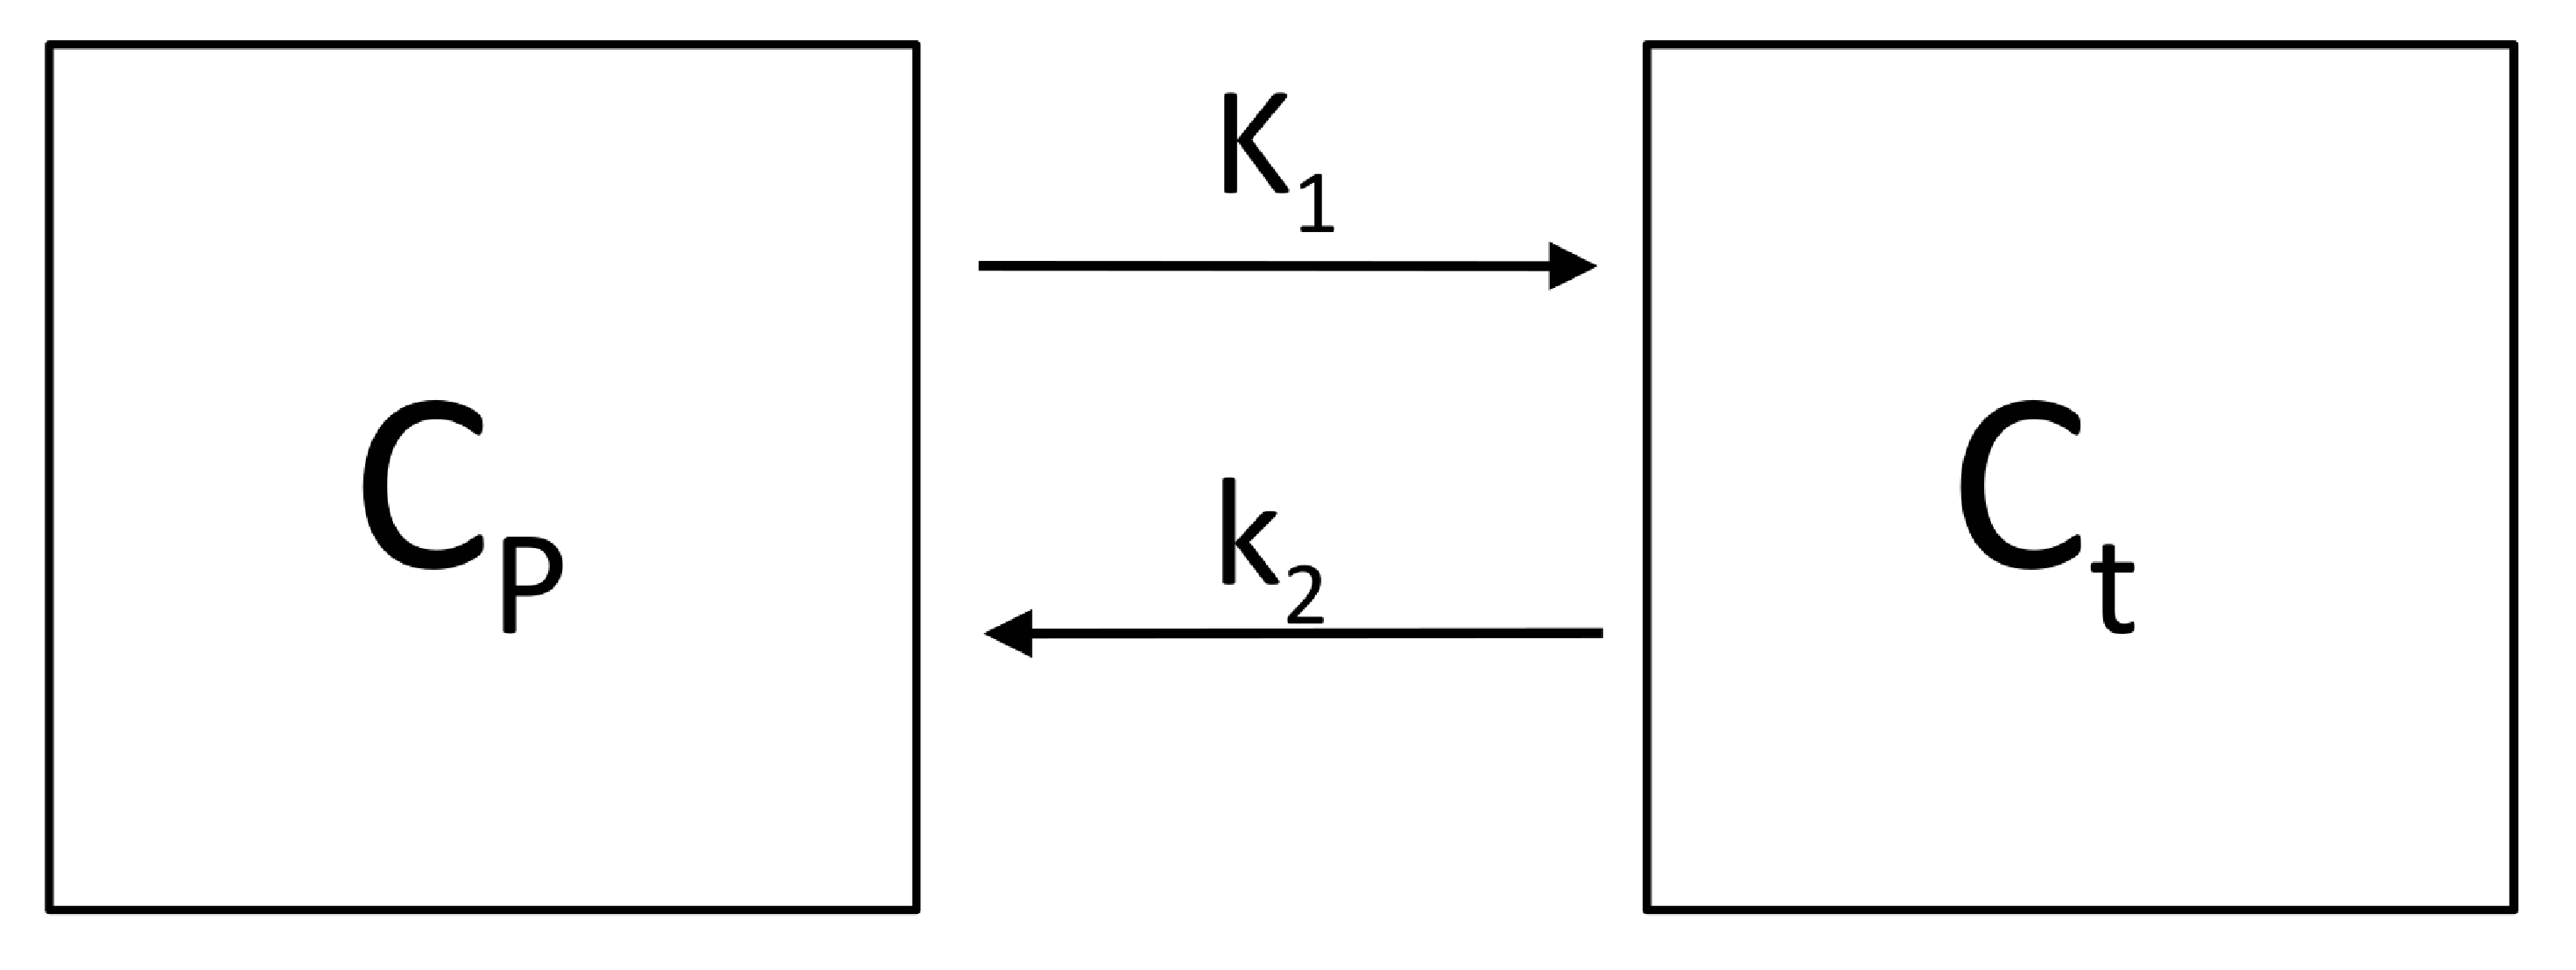
\includegraphics[width=0.4\columnwidth]{./figures/dynamic_1TCModel.eps}
  \caption{One tissue compartment Model with 2 parameters $K_1$ and $k_2$, where $C_p$ and $C_t$ are the concentration in plasma and tissue respectively.}
  \label{fig_1TCM}
\end{figure}

This model contains 3 parameters, including 2 rate constants, $K_1$ (unit: v/s/v, where v is a volume unit), $k_2$ (unit: s-1) and the arterial volume fraction in tissue ($V_a$), as described by the following equations :

\begin{equation}
C_{pet} ( t )    = C_t( t )    + V_a*C_p( t )
\label{eq_1TCM_CPET}
\end{equation}

\begin{equation}
dC_t( t ) / dt = K_1*C_p( t ) - k_2*C_t( t )
\label{eq_1TCM_CT}
\end{equation}

where $C_{pet}(t)$ denotes the image value in voxel for frame $t$, and $C_t$ and $C_p$ are activity concentration in tissue and plasma respectively. The model estimates $K_1$, $k_2$ and $V_a$ parametric images.
The input function ($C_p$), corresponding to the input plasma curve must be provided by the user.

\bigskip
This model can be initialized using either a configuration text file, or a list of options :

\subsubsection{configuration file:}
\label{sss_1TCM_cfile}

The file must be provided to the \textit{castor-recon} main executable using the following command-line options.

\bigskip
\verb| -dynamic-model _1TCM:/path/to/conf/file.txt|
\bigskip


\begin{itemize}

\item \textbf{Input\_function:}	(mandatory)
Enter the activity concentration values (kBq/v) of the plasma function ($C_p$) for each time frame ($tf$), on two successive lines, separated by ','. Time unit is seconds :

\bigskip
Input\_function: \\
\texttt{$C_{p,tf_1}$, $C_{p,tf_2}$, ..., $C_{p,tf_n}$}
\bigskip


\item \textbf{Integral\_input\_function:}

If the integral of the plasma input function is already computed, enter the activity concentration values of its coefficients ($I_{cp}$) for each time frame ($tf$), on two successive lines, separated by ','. Time unit is seconds.


\bigskip
Integral\_input\_function: \\
\texttt{$I_{cp,tf_1}$, $I_{cp,tf_2}$, ..., $I_{cp,tf_n}$}
\bigskip


NOTE: If not provided by the user, this integral will be estimated from the input function. Set the $Integral\_method$ flag below to select the method for TAC integration (default: WPO)).


\item \textbf{Optimisation\_method: x} (optional) Define the method to use for parameters estimation. Only least-squares methods are currently available to estimate $\theta$ = ($K_1$, $k_2$, $V_a$).

\begin{equation}
\widehat{\theta} = \frac{X'Wy}{X'WX}
\label{eq_NNLS}
\end{equation}

\begin{description}
\item $y$ = data vector
\item $X$ = model matrix ($C_p$, $I_{c_p}$, $C_{pet}$)
\item $W$ = weights vector (frame duration)
\end{description}

The different available Least-Square algorithms are

\begin{description}
\item 0 (default) = Iterative non-negative Least-Square. This code is derived from Turku PET center libraries, authors: Vesa Oikonen and Kaisa Sederholm.

Based on C.L. Lawson and R.J. Hanson, Solving Least Squares Problems.

(http://www.turkupetcentre.net/petanalysis/index.html).

NOTE: K1 estimated values could still be negative as they are computed from a substraction of the estimated NNLS parameters. Activity values will be kept to their original values for the voxels involved.
\item 1           = Standard Least Square (LS) optimisation. This algorithm can use Ridge Regression constraint (see below). If the estimated parameter values are negative, the activity value for the related voxels will be kept to their original number.
\end{description}


\item \textbf{Integration\_method:} x (optional) Define the method to use for TAC integration over the time samples.
\begin{description}
\item 0 (default) = Weighed parabola overlapping (WPO) (Z.Wang, D.Feng, Int. Sys. Sci 23 (1992), pp.1361-69)
\item 1           = Trapezoidal
\end{description}


\item \textbf{Ridge\_parameter:} Constant for Ridge Regression during Least-Square optimisation (only available with Least-Square algorithm and not NNLS ).
\textbf{Bounds} must be provided with the eponym options below in order to compute ridge weights and means for the new cost function:

\begin{equation}
\widehat{\theta} = \frac{X'Wy}{X'WX + t.Rw} + \frac{t.RwRm}{X'WX + t.Rw}
\label{eq_NNLS_ridge}
\end{equation}

\begin{description}
\item $y$ = data vector
\item $X$ = model matrix ($C_p$, $I_{c_p}$, $C_{pet}$)
\item $W$ = weights vector (frame duration)
\item $t$ = Ridge constant
\item $Rw$ = Ridge weights
\item $Rm$ = Ridge means
\end{description}



\item \textbf{Bounds:} (optional) Upper / Lower Bounds for each 3 parameters, to define for each parameter ridge means $mr=(Max+Min)/2$, and weights $wr=1/(Max-Min)^2$.

They must be provided as in the following syntax:

\bigskip
Bounds: $K_1Max$, $K_1Min$, $k_2Max$, $k_2Min$, $V_aMax$, $V_aMin$.
\bigskip

Default values:
\begin{description}
\item K1(Max,Min) = 0.1, 0.
\item K2(Max,Min) = 0.1, 0.
\item Va(Max,Min) = 1. , 0.
\end{description}

\item \textbf{VA\_image: path/to/image} (optional) Path to an interfile image containing the arterial volume fraction value in tissue for each voxel, only K1 and k2 rate constants will be estimated if such image is provided (Default: All parameters are estimated).

\end{itemize}




\subsubsection{Command line options:}
\label{sss_1TCM_list}

   The one-tissue compartment model initialization can be directly made from the command line options. The model just requires the samples of the plasma input curve, separated by commas:


\bigskip
\texttt{-dynamic-model \_1TCM,  $C_{p,tf_1}$, $C_{p,tf_2}$, ..., $C_{p,tf_n}$}
\bigskip



All other options will be set to default. The optimisation algorithm will be NNLS, the integration method for TAC will be WPO.
   
   
   
   
\newpage
\subsection{Parameters common to all dynamic model:} 
\label{ss_common_parameters}

The following keywords are optional and common to each dynamic model (Dynamic frame, Respiratory gating or Cardiac gating). They control the main functions dedicated to the estimation of the model parameters, and the re-estimation of the image using the model:

\begin{itemize}
\item \textbf{Number\_of\_iterations\_before\_image\_update: x}  

Set a number \textit{x} of iteration to reach before using the model to generate the images at each frames/gates (Default x ==  0) 
   
\item \textbf{No\_image\_update: x } 

If \textit{x} set to 1, the reconstructed images for the next iteration/subset are not reestimated using the model (the code just performs standard independent reconstruction of each frames/gates) (Default x = 0).       
          
\item \textbf{No\_parameters\_update: x} 

If set to 1, the parameters / functions of the model are not estimated with the image (this could be used to test The EstimateImageWithModel() function with specific user-provided parametric images) (Default x = 0).
   
\item \textbf{Save\_parametric\_images : x } 

Enable (1)/Disable(0) saving parametric images on disk (Default x == 1)  

\item \textbf{Save\_blacklisted\_voxels\_images : x } 

Enable (1)/Disable(0) saving blacklisted voxels images on disk (Default x == 0)  

\item \textbf{Mask : x } 

Path to an interfile image containing a mask indicating if the model must be applied (1) or not (0) in each voxel (Default: model applies everywhere)  

\end{itemize}


\bigskip
\section{castor-imageDynamicTools toolkit}
\label{s_dmodel_toolkit}

This utility can be used to apply any of the dynamic model implemented in CASToR over a set of dynamic images. This can be used either to test a dynamic model, or to apply the model as a post-reconstruction processing. 

\bigskip
As with \textit{ castor-recon}, the dynamic model should be called with \textit{-dynamic-model}. The set of dynamic image (either a dynamic image, or the metaheader of a set of dynamic images), or a dynamic image must be called with the \textit{-i} option. 

\bigskip
Please look at section 8 of the general documentation to have a description of the dynamic image interfile format. Additionally, the \textit{-h} option will display all command line options provided by this utility.


\clearpage
%---------------------------------------------------------------------------------------------------------------------------------------------------------------
\section{Add your own dynamic model}
\label{section_add_own_dynamic_model}

\subsection{Basic concept}


The addition of a new dynamic model mostly require to implement these two functions. Note that these functions can be individually enabled/disabled depending on the values of some parameters implemented by \textit{vDynamicModel} specific to vDynamicModel as specified in section \ref{ss_common_parameters}.


The addition of a new image-based dynamic model require to build a specific class that inherits from the abstract class \textit{vDynamicModel}. Then, one just has to implement a set of pure virtual functions for the initialization and application of the model. Please refer to the \textit{CASToR\_HowTo\_\_add\_new\_modules.pdf} guide in order to fill up the mandatory parts of adding a new module; namely the auto-inclusion mechanism, the interface-related functions and the management functions. To ease the implementation, a template class is provided in the source code and already implements all the squeleton. Basically, one will have to change the name of the class and fill the related functions up in his own code. The actual files are \textit{include/dynamic/iDynamicModelTemplate.hh} and \textit{src/dynamic/iDynamicModelTemplate.cc} and are already part of the source code. Right below are some instructions to help fill the specific pure virtual projection functions of a dynamic model.
\bigskip



\subsection{Implementation of the dynamic model functions}

Several mandatory functions should be implemented (or return an error by default) in a new dynamic model class :

\begin{description}
\item \textbf{ShowHelp()}: Simply output some help and guidance to describe what the dynamic model does and how to use it.

\item \textbf{ReadAndCheckOptionsList()}: Implement here the reading of any options specific to this dynamic model passed through the argument \texttt{const string\& a\_listOptions}. The user can make use of the \textit{ReadStringOption()} function to parse the list of parameters. If the function is not mandatory (e.g initialization of the model using a file is required rather than with command-line parameters), just send an error message and return 1.

\item \textbf{ReadAndCheckConfigurationFile()}: Implement here the reading of any configuration file specific to this dynamic model, passed through the argument \texttt{const string\& a\_fileOptions}. The user can make use of the \textit{ReadDataASCIIFile()} function to read data from a file. If the function is not mandatory (e.g initialization of the model using command line options is required rather than with a file), just send an error message and return 1.

\item \textbf{CheckParameters()}: Use this function to check if the private parameters of your class have correctly been initialized. It might be a good idea to initialize all private parameters in the constructor with default erroneous value to properly check their initialization.

\item \textbf{InitializeSpecific()}: Use this function to Instanciate/Initialize any member variables/arrays after the parameters have been checked in the previous function.
  
\item \textbf{EstimateModelParameters()}: The estimation of the model parameters and parametric images must be implemented here, with the help of any private functions if required. The \textit{ap\_ImageS} parameter allows to access the image matrices in the oImageSpace class. The current estimation of the image \textit{m4p\_image} can be accessed from there. It contains 4 dimensions in order to access to any dynamic level : 

$ap\_ImageS->m4p\_image[fr][rg][cg][v]$ \\
fr = time frames \\
rg = respiratory gates \\
cg = cardiac gates \\
 v = actual voxel of the 3D volume

\item \textbf{EstimateImageWithModel()}: This function can be used to generate the serie of dynamic images from the model (i.e, the image matrix $ap\_ImageS->m4p\_image$), after estimation of the model parameters in EstimateModelParameters(). It is called right after EstimateModelParameters()

All information and the tools needed to implement these functions are fully described in the template source file \textit{src/dynamic/iDynamicModelTemplate.cc}, so please refer to it.

\end{description}





\clearpage
\section{Meta-data command line options}
\label{section_Meta-data command line options}
List of the different set of options related to image-based dynamic models :
\begin{itemize}
\item \textbf{-frm} \textit{path/to/file}: Give the framing details for the reconstruction where 'list' is a list of frame start times, separated with commas. Duration for each frame can also be specified using a colon after the frame start time. When no duration is specified for a frame, the duration will be set equal to the difference between the start of this frame and the next one. It is mandatory to specify the duration of the last frame. For example '-frm start1:duration1,start2,start3:duration3'. Add 's' or 'm' to specify if values are seconds or minutes (seconds is the default if none provided). Maximum precision of frames is milliseconds. (default: 1 frame of the whole input file duration).           
\item \textbf{-g} \textit{path/to/file}: Give a text file defining the gating of the dynamic data. The number of gates, and number of events in each gate, must be provided using different keywords :
\begin{description}
\item \texttt{nb\_respiratory\_gates}: number of respiratory gates in the data
\item \texttt{nb\_events\_respiratory\_gates}: enter the number of events within each gate, separated by commas. If the data contains several frame (dynamic acquisition), the data splitting of each frame should be entered on a new line (1 line by frame).
\item \texttt{nb\_cardiac\_gates}: number of cardiac gates in the data
\item \texttt{nb\_events\_cardiac\_gates}: enter the number of events within each gate, separated by commas. If the data contains several frame (dynamic acquisition), the data splitting of each frame should be entered on a new line (1 line by frame).
\item \texttt{duration\_gate}: (optional) enter the duration (seconds) of each gate, separated by commas. If the data contains several frames (dynamic acquisition), the gate durations of each frame should be entered on separate line (1 line by frame).
\end{description}
\item \textbf{-aic} \textit{path/to/file}: This option will enable the Creation of Patlak Basis functions for direct Patlak Reconstruction (For nested recon look in -help-dynamic-model ). Provide text file with the Arterial Input Curve data points and time points, in two different horizontal lines starting with 'AIC\_time\_points:' and 'AIC\_data\_points:' to indicate which dataset corresponds to each line. Values must be separated by commas. Also provide a value of the total number of data points, on a new line starting with 'AIC\_number\_of\_points:'.
\item \textbf{-qdyn} \textit{path/to/file}: Provide a text file containing quantitative factors specific to dynamic frames, respiratory or cardiac gates. The file should provide factors with the keywords 'FRAME\_QUANTIFICATION\_FACTORS' and 'GATE\_QUANTIFICATION\_FACTORS'. The number of factors must be consistent with the number of frames/gates. If the data contains several frames and gates, the gate quantification factors should be entered on a separate line for each frame 
\item \textbf{-help-dynamic-model} \: Print out specific help about dynamic model
\end{itemize}



%---------------------------------------------------------------------------------------------------------------------------------------------------------------
%---------------------------------------------------------------------------------------------------------------------------------------------------------------
%---------------------------------------------------------------------------------------------------------------------------------------------------------------
%          R E F E R E N C E S
%---------------------------------------------------------------------------------------------------------------------------------------------------------------
%---------------------------------------------------------------------------------------------------------------------------------------------------------------
%---------------------------------------------------------------------------------------------------------------------------------------------------------------
\bibliographystyle{IEEEtran} 
%\bibliographystyle{apalike} 
\bibliography{CASToR_general_documentation}

% that's all folks
\end{document}
